% Beamer template
% Author: Ozgur Taylan TURAN
% Delft University of Technology

\documentclass[aspectratio=169]{beamer}
% PACKAGES
\usepackage[english]{babel}
\usepackage{graphicx}
\usepackage{animate}
%\usepackage{calc}
\usepackage{calligra}
\usepackage[absolute,overlay]{textpos}
\usepackage[T1]{fontenc}
%\usefonttheme{serif}
\usefonttheme{professionalfonts}
\usepackage{amsmath}
\usepackage{palatino}
\usepackage{mathpazo}
\usepackage{graphicx}
%\usepackage{subfig}
\usepackage{tikz}
\usetikzlibrary{shapes,arrows}
\usepackage{xcolor}
\usepackage[T1]{fontenc}
%\usefonttheme{serif}
%\usepackage{titling}
\usepackage{graphicx}
%\usepackage{subfig}
%\usepackage{tikz}
%\usetikzlibrary{shapes,arrows}
\usepackage{mathtools}
\usepackage{cancel}
% CUSTOM PACKAGES
\usepackage{/home/taylanot/texmf/tex/beamerthemetot}
\input{/home/taylanot/texmf/presentation/tune.tex}

 % COVER PAGE INFO   
\newcommand{\mytitle}{\color{White}\huge{\textbf{Shallow Meta-Learning Strategies \& Applications}}}
\newcommand{\mysubtitle}{\color{Pink}\huge{\textbf{Yearly Progress Meeting \#1}}}
\newcommand{\mig}{\color{Pink}\huge{\textbf{Miguel's Departure}}}
\newcommand{\work}{\color{Pink}\huge{\textbf{WORK}}}
\newcommand{\reflect}{\color{Pink}\huge{\textbf{Reflection}}}
\newcommand{\thx}{\color{Pink}\huge{\textbf{Thanks!}}}
\newcommand{\myauthor}{\color{White}\textcalligra{\LARGE Ozgur Taylan Turan}}
\newcommand{\authorlabel}{\small O.T. Turan}
\author{\authorlabel}

\setlength\bibitemsep{0.3cm} % space between entries in the reference list
\renewcommand{\bibfont}{\normalfont\scriptsize}
\renewcommand{\cite}[1]{\footnote<.->[frame]{\fullcite{#1}}}
\setbeamertemplate{bibliography item}{}
\bibliography{../../../../references/LabTalk.bib}


\begin{document}
% COVER PAGE
{
\def\beamer@entrycode{\vspace*{-\headheight}}
\setbeamertemplate{frametitle}[default][center]
\setbeamertemplate{navigation symbols}{}
\usebackgroundtemplate{
\includegraphics[width=\paperwidth,height=\paperheight]{cover/coverart.pdf}}

\begin{frame}[plain] 

\begin{minipage}{\textwidth}
	\centering{\mytitle} \\
	%\vspace{1cm}
	%\centering{\mysubtitle} \\
	\vspace{1cm}
	\centering{\color{White}November 15, 2021} \\
	\vspace{1cm}
	\centering{\myauthor}\\
\end{minipage}
\end{frame}
}


%\begin{frame}{Outline}
%  \begin{itemize}
%    \item Miguel
%    \item Past Work
%    \item Current \& Upcoming Work
%    \item Reflection
%    \item Carrier Opportunities
%  \end{itemize}
%\end{frame}

\begin{frame}
  \centering
  \mig
\end{frame}

\section{Miguel's Departure}

\begin{frame}{+/-}
  \begin{minipage}{0.5\textwidth}
    \color{Pink} Positives
    \begin{itemize}
      \item Reduced stress
      \item Reduced internal questioning
      \item Increased mental and physical health
    \end{itemize}
  \end{minipage}%
  \begin{minipage}{0.5\textwidth}
  \only<2>
  {
    \color{Pink} Negatives
    \begin{itemize}
      \item Reformulation of the project 
      \item Concluding the on going works
      \item Lingering ethical issues
    \end{itemize}
  }
  \end{minipage}
\end{frame}

\section{Work}

\begin{frame}
  \centering
  \work
\end{frame}


\begin{frame}{Past Work}
  \begin{minipage}{\textwidth}
    \color{Pink} When MAML Learns Quick Does It Generalize Well? [BNAIC/BeNeLearn]
    \begin{itemize}
      \item First paper
      \item Experienced the full cycle
    \end{itemize}
  \end{minipage}
  \begin{minipage}{\textwidth}
  \only<2>
  {
    \color{Pink} Cooperative Data-Driven Modeling [ArXiv/ICLR/CMJ]
    \begin{itemize}
      \item First collaboration 
      \item Not really satisfied 
    \end{itemize}
  }
  \end{minipage}
\end{frame}

\begin{frame}{Side Projects}
  \begin{minipage}{0.5\textwidth}
  \only<1-2>
  {
    \color{Pink} Civil Engineering Connections
    \begin{itemize}
      \item MSc student (Gaussian Process)
      \item Paper?
    \end{itemize}
  }
  \only<3-4>
  {
    \color{Pink} Own ML Library in C++
    \begin{itemize}
      \item Fast learning curve generation
      \item Data and code management
    \end{itemize}
  }
  \end{minipage}%
  \begin{minipage}{0.5\textwidth}
  \only<2>
  {
    \color{Pink} UQ with Yuko
    \begin{itemize}
      \item Material Science UQ application
      \item Paper?
    \end{itemize}
  }
  \only<4>
  {
    \color{Pink} Meta-Learning material science problems
    \begin{itemize}
      \item Low-hanging fruit
      \item Paper?
    \end{itemize}
  }
  \end{minipage}
\end{frame}

\begin{frame}{Future Work}
  \begin{minipage}{0.5\textwidth}
    \color{Pink} Semi-Parameter Kernel Ridge 
    \begin{itemize}
      \item Second Paper -> Application on Learning Curves (with Tom)
      \item Third Paper -> Kernel Learning/Construction
    \end{itemize}
  \end{minipage}%
  \begin{minipage}{0.5\textwidth}
  \only<2>
  {
    \color{Pink} Bayesian Shallow Meta-Learning
    \begin{itemize}
      \item Final Paper
    \end{itemize}
  }
  \end{minipage}
\end{frame}

\begin{frame}{Planning Project}
  \centering
  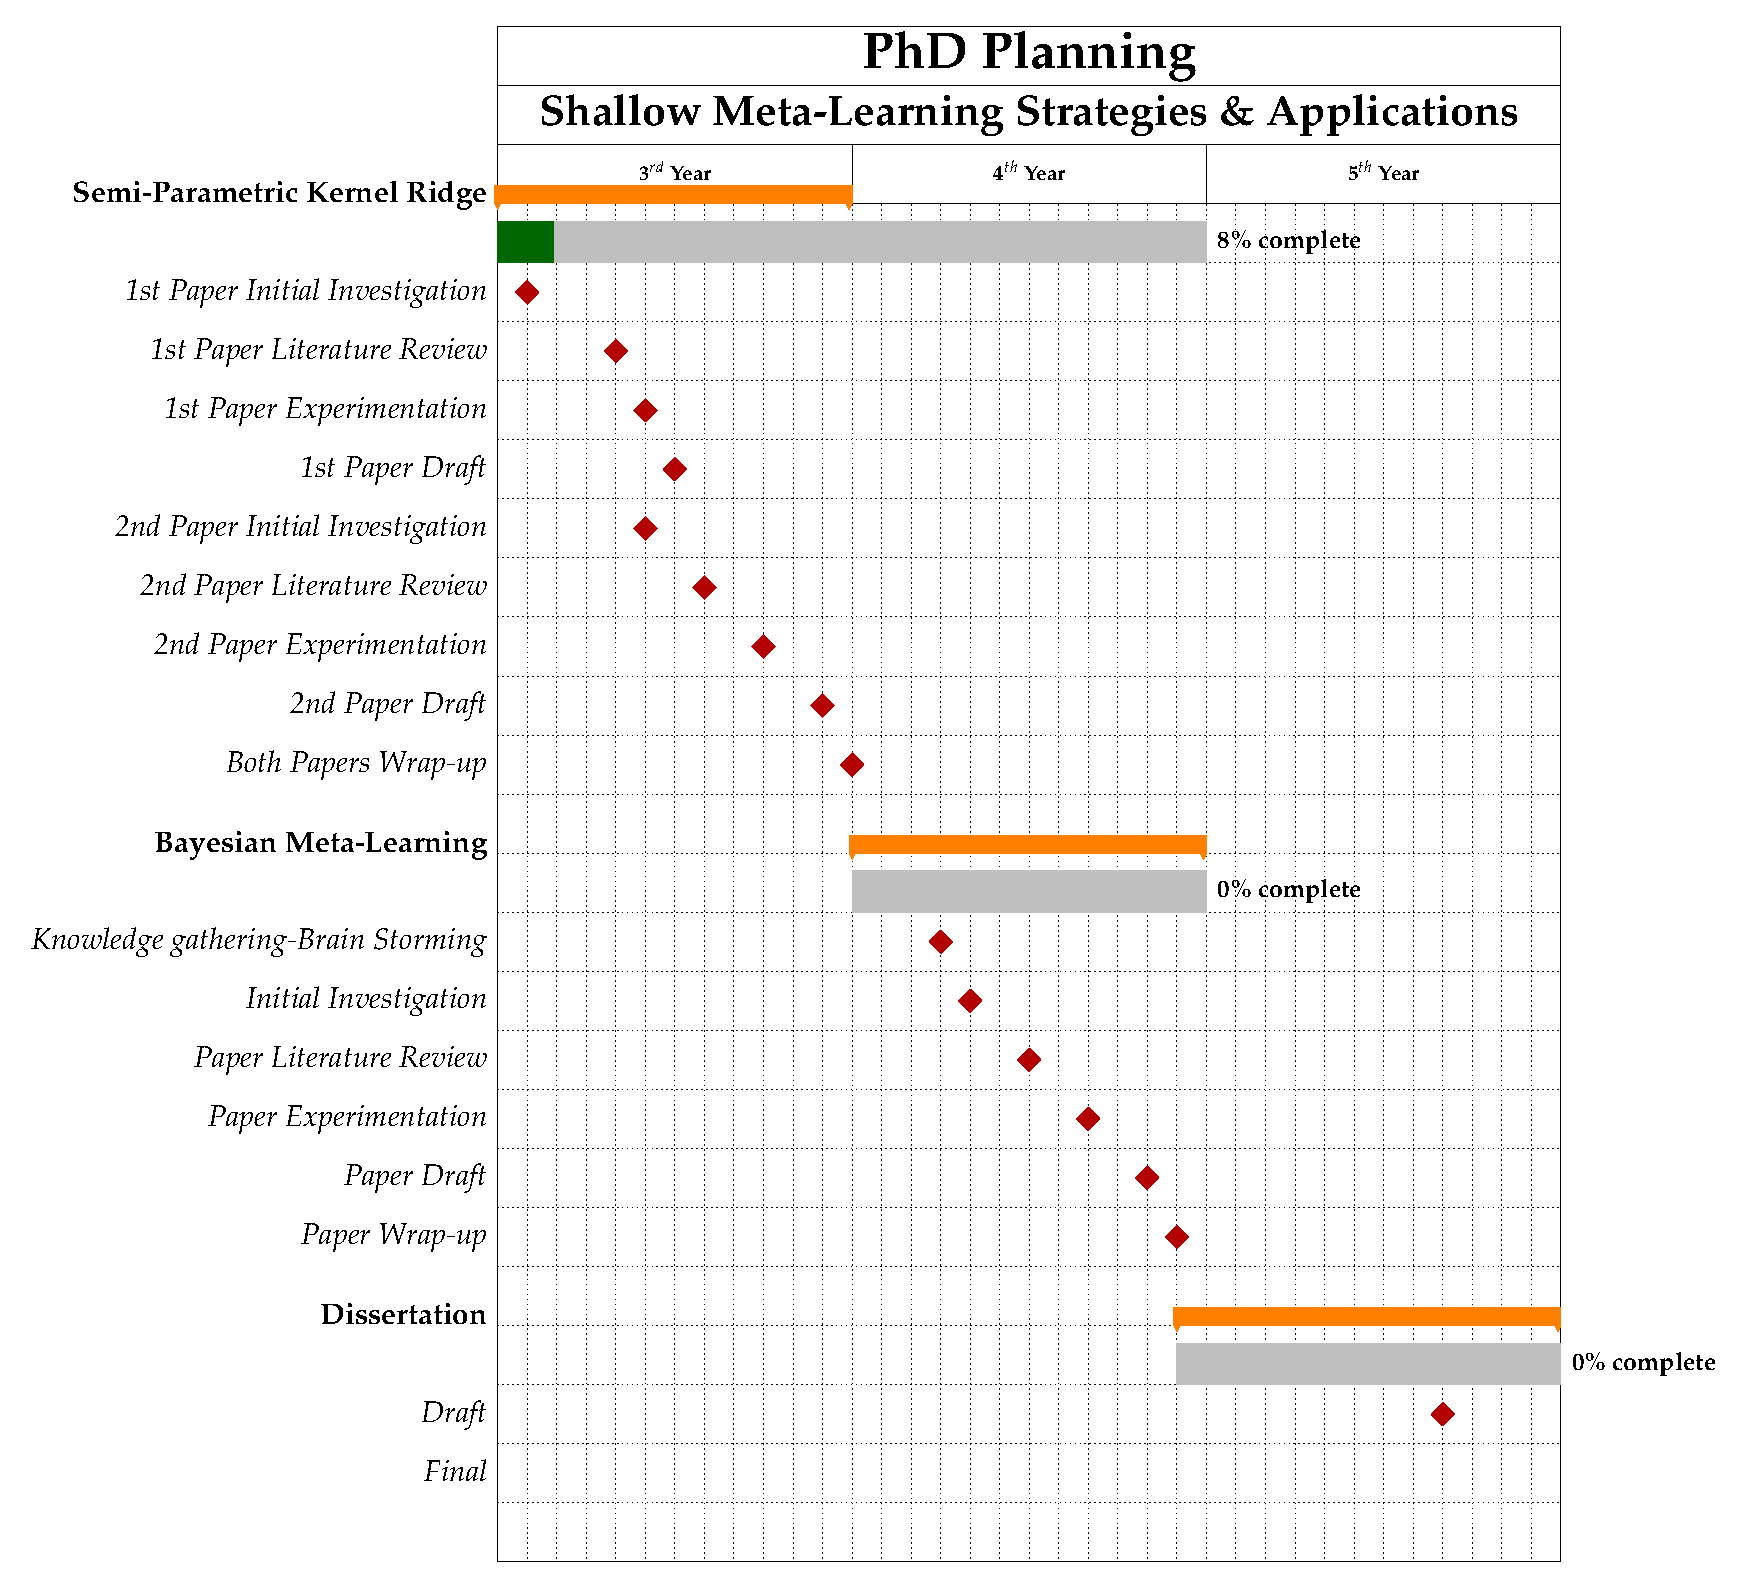
\includegraphics[width=0.5\textwidth]{figures/plan.pdf} % 
\end{frame}


\begin{frame}{Planning-Transferable Skills}
  \begin{minipage}{0.5\textwidth}
  \centering
  \begin{tabular}{ c|c|c } 
    \textbf{Lecture} & \textbf{Credit}& \textbf{Status} \\ 
    \hline
    Start-A& 0.5 & + \\ 
    Start-B& 1.0 & + \\ 
    Start-C& 0.5 & + \\ 
    Mental Fitness& 1.0 & + \\ 
    Standing up for yourself & 1.0 & + \\ 
    Analytical storytelling & 2.5 & + \\ 
    Work smarter stress less & 2.0 & + \\ 
    \hline
  \end{tabular}
  \end{minipage}%
  \begin{minipage}{0.5\textwidth}
  \centering
  \begin{tabular}{ c|c|c } 
    \textbf{Lecture} & \textbf{Credit}& \textbf{Status} \\ 
    \hline
    Speedreading & 1.5 & + \\ 
    Time management& 0.5 & + \\ 
    Poster Day& 1.0 & + \\ 
    Teaching train...& 1.0 & + \\ 
    Dutch & 3.0 & + \\ 
    \color{Pink}Data Management & 1.5 & - \\ 
    \color{Pink}Looking for work in NL & 1.0 & - \\ 
    \hline
  \end{tabular}
  \end{minipage}
\centering
  Credits :15.5/18 (Needed Credits:15)
\end{frame}

\begin{frame}{Planning-Discipline Related Skills}
  \centering
  \begin{tabular}{ c|c|c } 
    \textbf{Lecture} & \textbf{Credit}& \textbf{Status} \\ 
    \hline
    Machine Learning-I& 5.0 & + \\ 
    Deep Learning & 5.0 & + \\ 
    \color{Pink}Summer School & 5.0 & - \\ 
    \hline
  \end{tabular}

    Credits : 10/15 (Needed Credits:15)
  \begin{itemize}
    \item Will try to go to ProbAI/ELLIS Summer School on Prob. ML (either this year or next)! 
  \end{itemize}
\end{frame}

\begin{frame}{Planning-Research Related Skills}
  \centering
  \begin{tabular}{ c|c|c } 
    \textbf{Lecture} & \textbf{Credit}& \textbf{Status} \\ 
    \hline
    \color{Pink}Paper Review  & 1.0 & Miguel(+/-)? \\ 
    \color{Pink}Writing Conference Paper & 1.0 & BNAIC(+/-)? \\ 
    \color{Pink}Writing Journal Article & 3.0 & Mechanics(+/-)? \\ 
    \color{Pink}Supervise MSc & 4.0 & Civil Engineering(+/-)? \\ 
    \color{Pink}Supervise BSc & 4.0 &  2xCapstone/2xBScProject(+/-)?\\ 
    \color{Pink}Exam Prep. & 4.0 & Helping(+/-)? \\ 
    \color{Pink}Lab Prep. & 4.0 & Helping(+/-)? \\ 
    \color{Pink}Course & 4.0 & Helping(+/-)? \\ 
    \hline
  \end{tabular}

  \centering
    Credits : ?/23 (Needed Credits:15)
  \begin{itemize}
    \item A bit confused about these!
  \end{itemize}
\end{frame}

\section{Reflection}

\begin{frame}
  \centering
  \reflect
\end{frame}


\begin{frame}{Self Reflection}
  \only<1>
  {
    \begin{itemize}
      \item Departure of Miguel
      \item Personal life struggles
      \item But, tones of relief and comfort at working environment
      \item COVID effects are wearing-off 
    \end{itemize}
  }
  \begin{minipage}{0.5\textwidth}
    \only<2-3>
    {

    \color{Pink} Getting Confident
    \begin{itemize}
      \item Working with others
      \item Being part of a group
      \item Scientific Knowledge
      \item Presenting, talking, taking responsibility 
      \item Research skills
    \end{itemize}
  }
  \end{minipage}%
  \begin{minipage}{0.5\textwidth}
  \only<3>
  {
    \color{Pink} Needs more attention
    \begin{itemize}
      \item Teaching, supervision, coaching
      \item Self-supervision
      \item Writing 
    \end{itemize}
  }
  \end{minipage}
\end{frame}

\begin{frame}{Supervision Reflection}
  \begin{minipage}{0.5\textwidth}
    \color{Pink} Good Sides 
    \begin{itemize}
      \item Tones of ideas and feedback
      \item Lots of freedom 
      \item Environment facilitating creativity
    \end{itemize}
  \end{minipage}%
  \begin{minipage}{0.5\textwidth}
  \only<2>
  {
    \color{Pink} Bad Sides
    \begin{itemize}
      \item Tones of ideas and feedback
    \end{itemize}
  }
  \end{minipage}
\end{frame}

\begin{frame}{Carrier Perspectives}
  \begin{itemize}
    \item Would like to stay in academia!
    \item A bit scared of not finding a position!
    \item Trying out an internship/visit industry/academia for a year after getting a Dutch Passport!
  \end{itemize}
\end{frame}

\begin{frame}
  \centering
  \thx
\end{frame}


%%%%%%%%%%%%%%%%%%%%%%%%%%%%%%%%%%%%%%%%%%%%%%%%%%%%%%%%%%%%%%%%%%%%%%%%%%%%%%%
% IF NEEDED
%%%%%%%%%%%%%%%%%%%%%%%%%%%%%%%%%%%%%%%%%%%%%%%%%%%%%%%%%%%%%%%%%%%%%%%%%%%%%%%

\begin{frame}{View of the Project-Before}
  \centering
  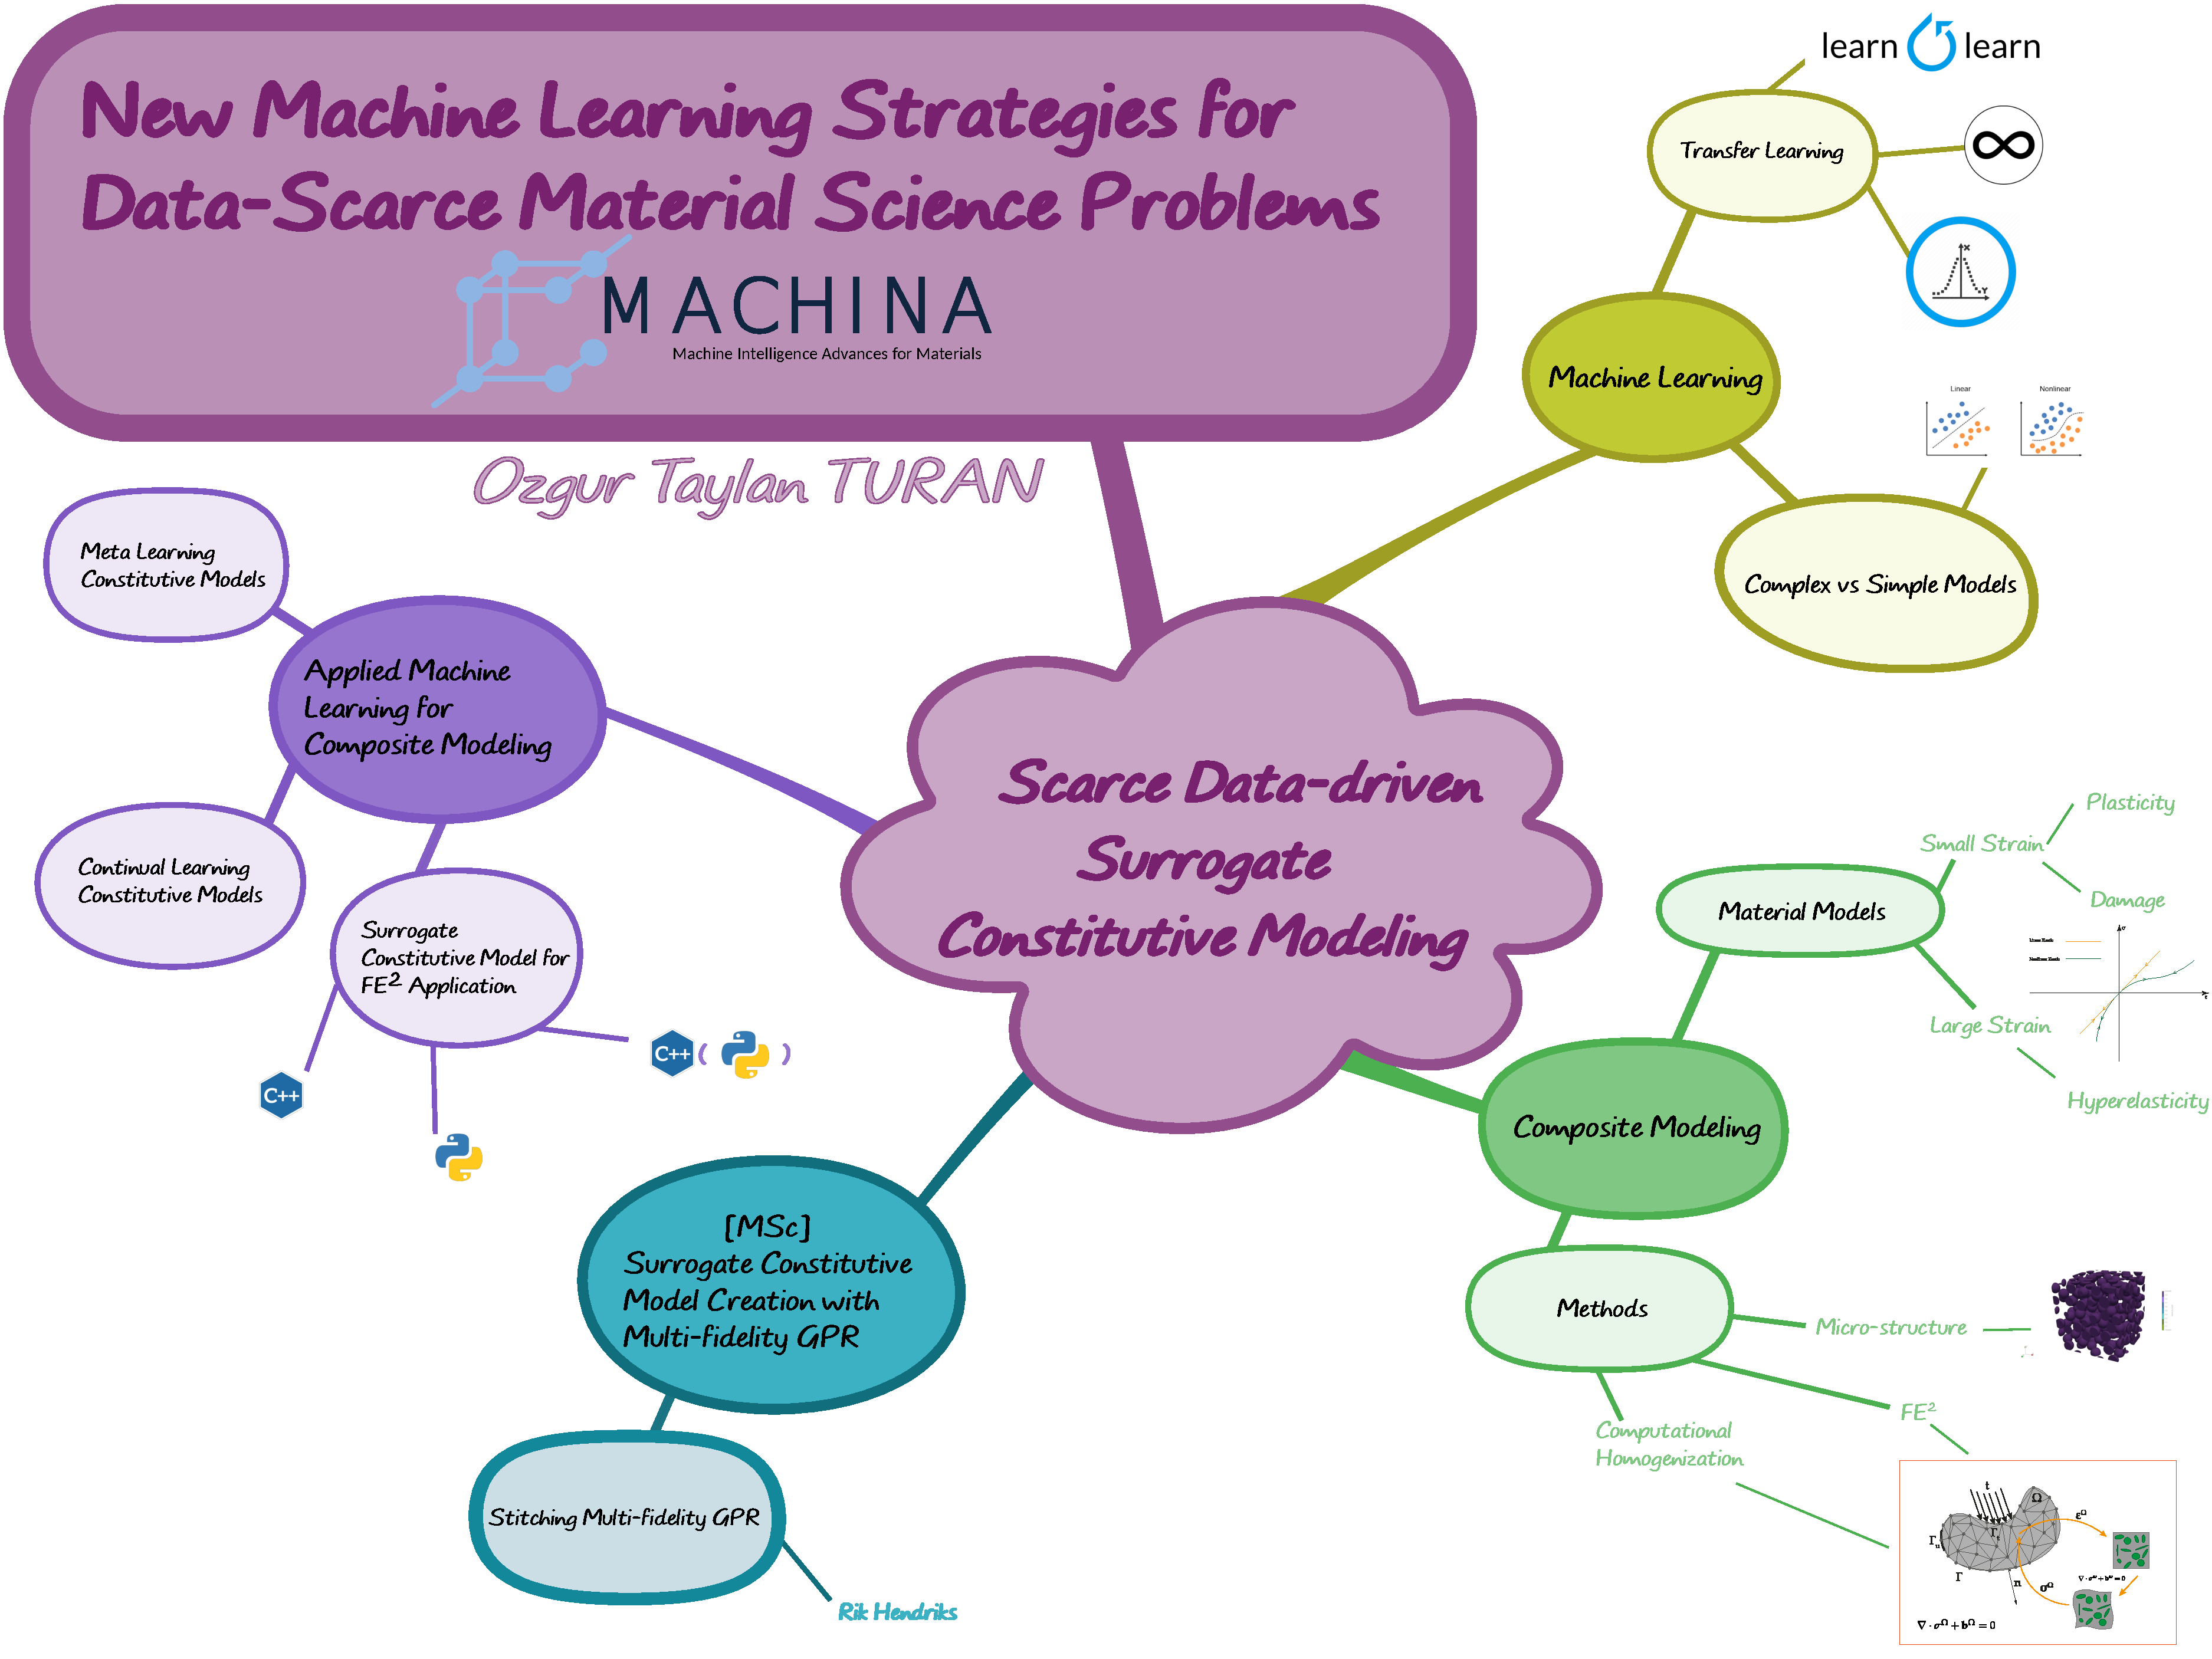
\includegraphics[width=0.6\textwidth]{figures/mindmap.pdf}
\end{frame}

\begin{frame}{View of the Project-After}
  \centering
  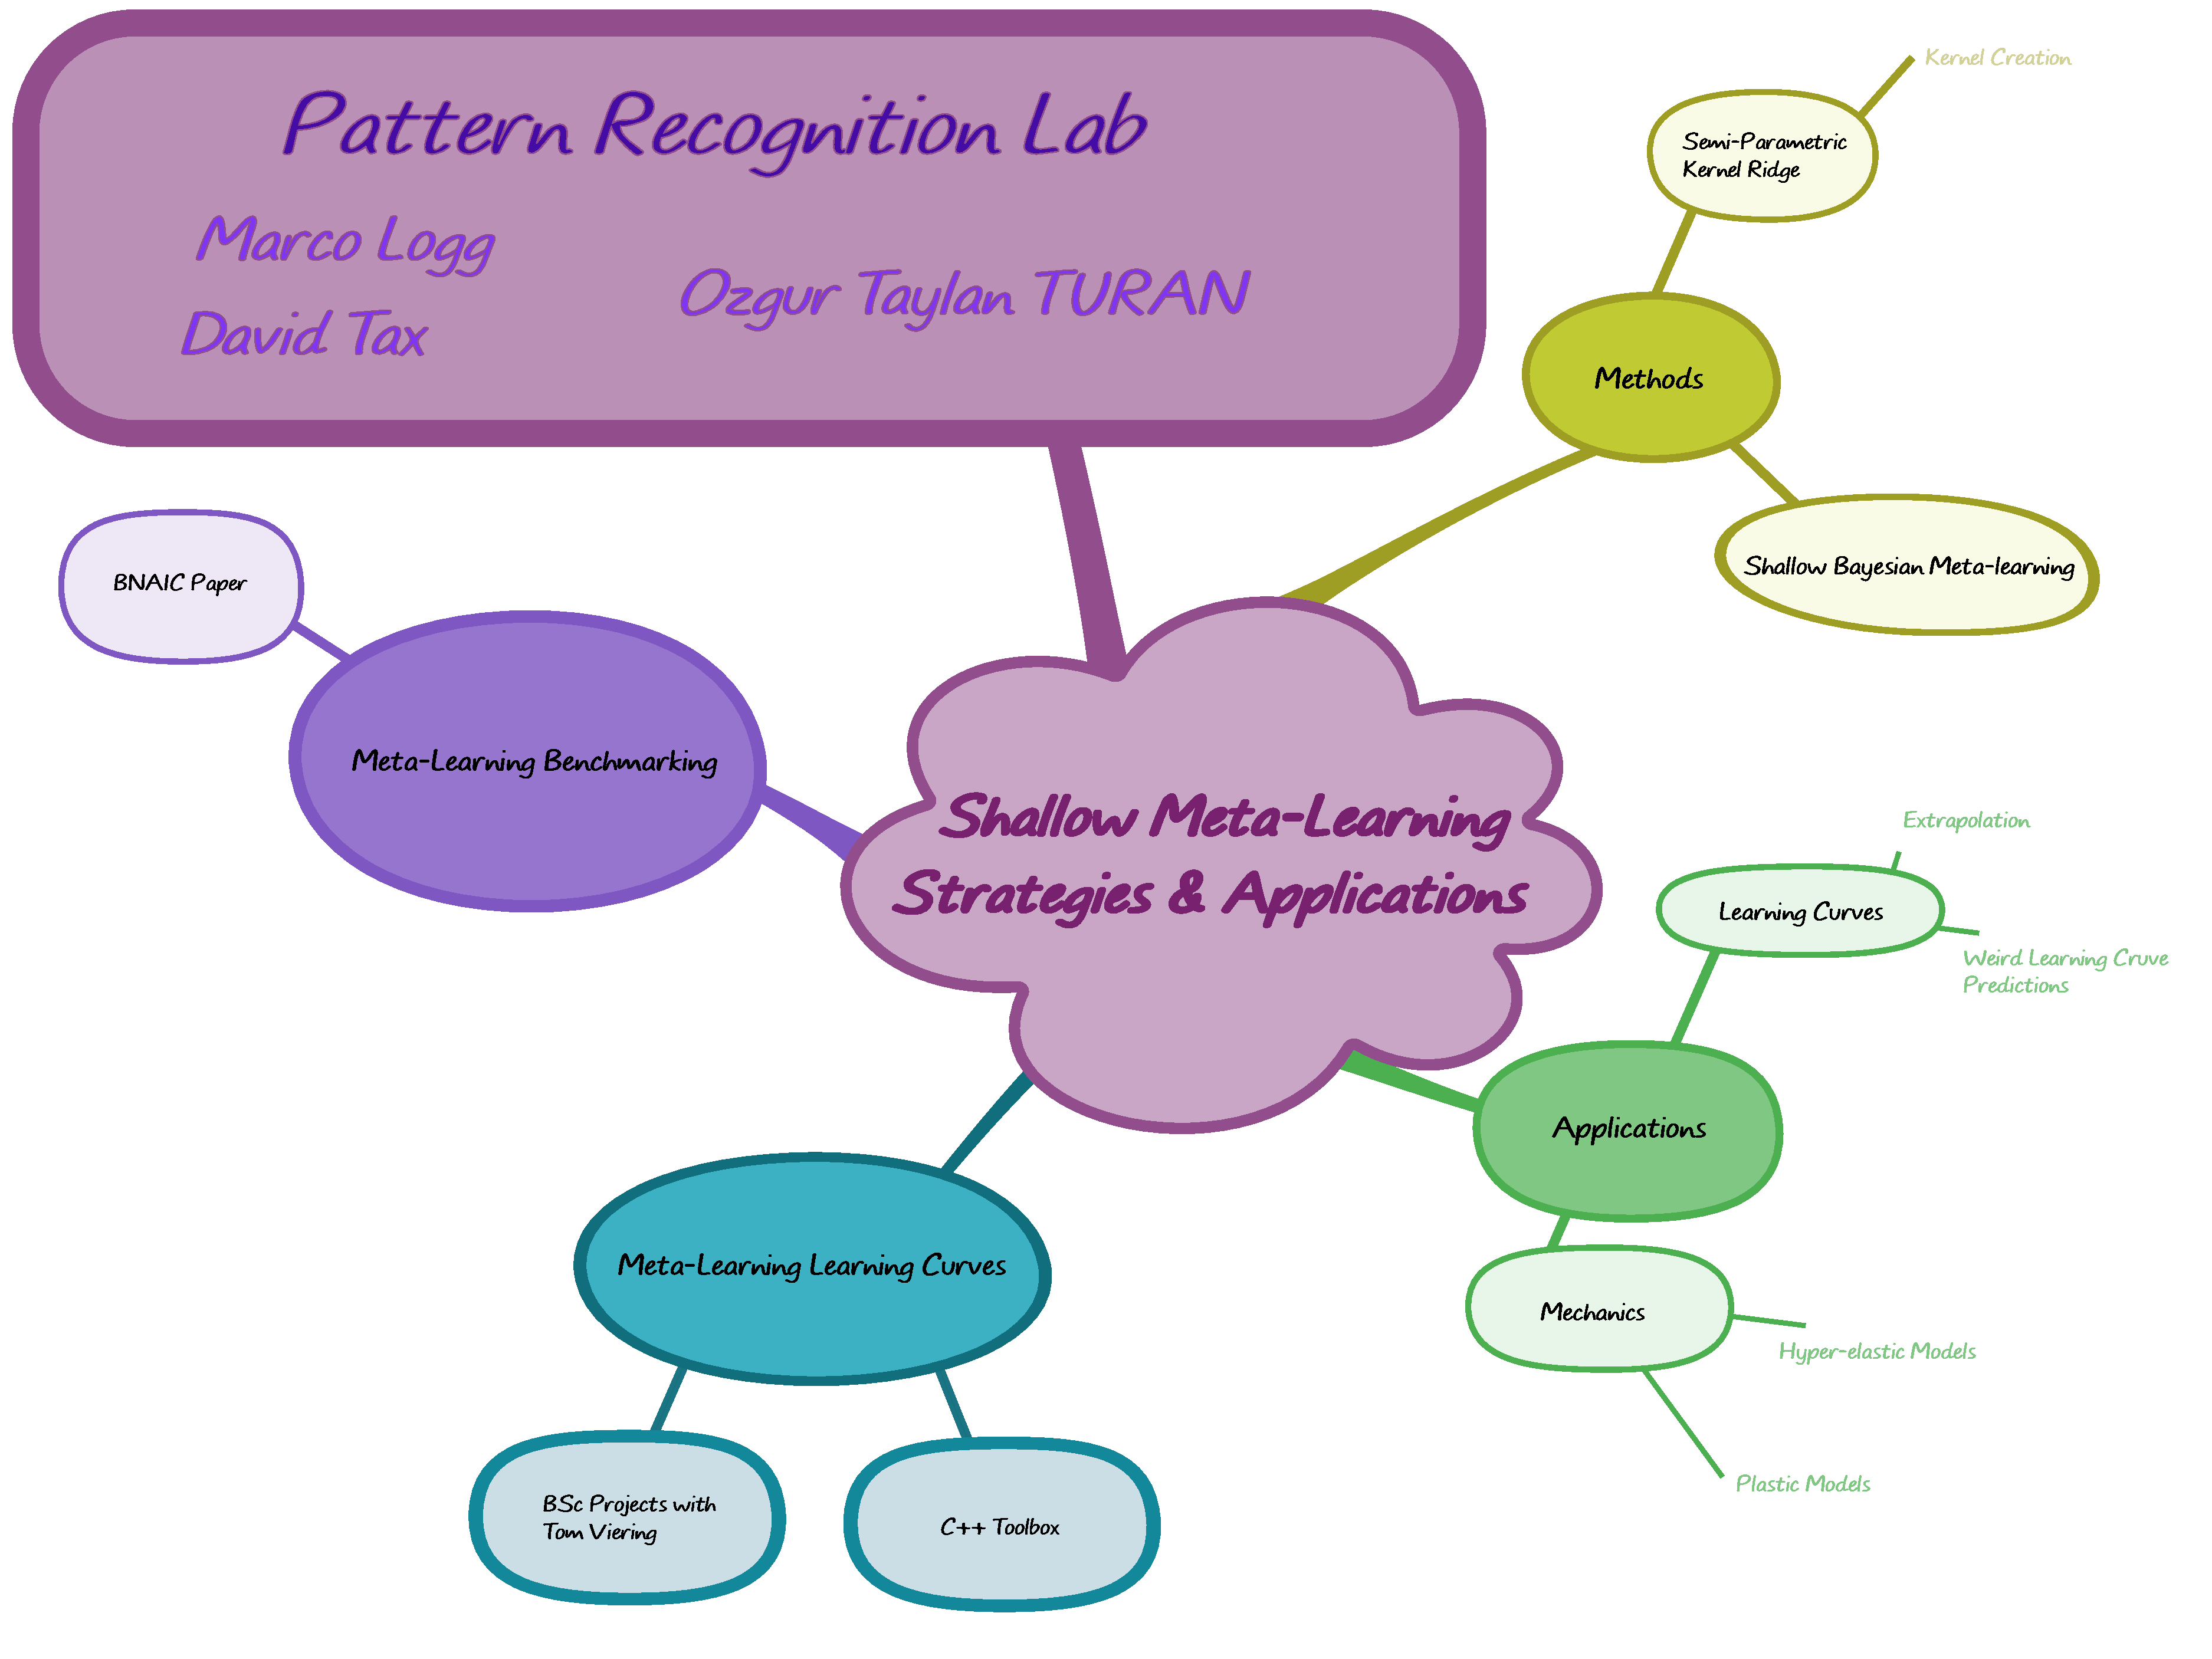
\includegraphics[width=0.6\textwidth]{figures/mindmap_new.pdf}
\end{frame}



\end{document}
